\section{Exploration des données}

\subsection{Format des données}

Le jeu de données d'apprentissage est constitué de \textbf{4410 patches} provenant de 5 puits distincts (puits 2, 3, 4, 5 et 6). Les données brutes, initialement vectorisées et présentant une hétérogénéité de résolution ($160 \times 272$ ou $160 \times 160$), sont annotées selon trois classes : \textbf{Background} (0), \textbf{Casing} (1) et \textbf{TIE} (2).

\subsection{Distribution et déséquilibre des données}

L'analyse exploratoire révèle une double asymétrie structurelle :
\begin{enumerate}
    \item \textbf{Disparité géographique} : La répartition des échantillons par puits varie d'un facteur 1 à 5 (300 à 1600 patches), induisant un risque de sur-représentation des formations géologiques dominantes.
    \item \textbf{Déséquilibre de classes} : Les structures d'intérêt sont largement minoritaires (\textbf{Casing} : 9\%, \textbf{TIE} : 6\%) face au fond (\textbf{Background} : 85\%). Ce ratio de 15:1 expose le modèle au risque de convergence triviale vers la classe majoritaire.
\end{enumerate}

\begin{figure}[ht]
    \centering
    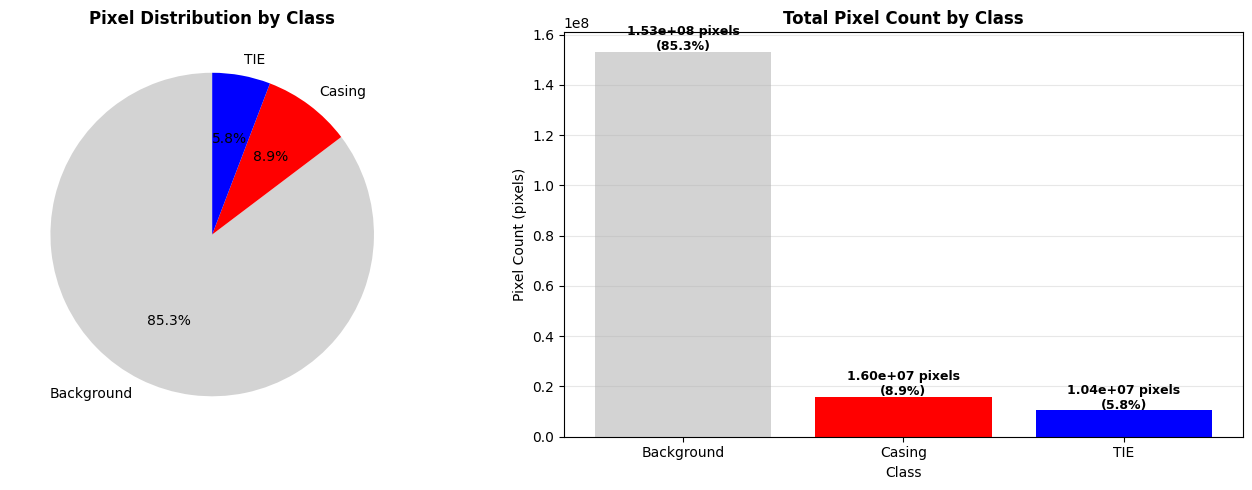
\includegraphics[width=0.5\textwidth]{Configuration/distribution_classes.png}
    \caption{Distribution des classes dans le dataset}
    \label{fig:class_distribution}
\end{figure}

Pour neutraliser ces biais, nous avons adopté une stratégie combinant pondération des classes (\textit{class weights}) dans la fonction de coût, augmentation synthétique des données et expérimentation sur la fonction de perte.

\subsection{Pipeline de prétraitement
    et justification des techniques}

Le pipeline de prétraitement s'articule autour de trois opérations fondamentales garantissant la qualité des entrées du réseau de neurones :

\begin{enumerate}
    \item \textbf{Standardisation dimensionnelle} : Les images sont redimensionnées uniformément à $160 \times 160$ pixels. Une stratégie d'interpolation différenciée est appliquée : bilinéaire (\texttt{INTER\_LINEAR}) pour les images d'intensité afin de préserver la continuité du signal, et au plus proche voisin (\texttt{INTER\_NEAREST}) pour les masques de segmentation afin de garantir l'intégrité des classes discrètes.
    \item \textbf{Intégrité numérique} : Les éventuelles valeurs défaillantes (NaN) générées par les transformations géométriques sont détectées et imputées par 0 (signal nul).
    \item \textbf{Normalisation radiométrique} : L'intensité des pixels est normalisée linéairement dans l'intervalle $[0, 1]$ selon $\tilde{x} = \frac{x - x_{min}}{x_{max} - x_{min}}$. Cette étape est indispensable pour homogénéiser la dynamique des entrées et faciliter la convergence de l'optimiseur.
\end{enumerate}

Voici un exemple illustré :

\begin{figure}[ht]
    \centering
    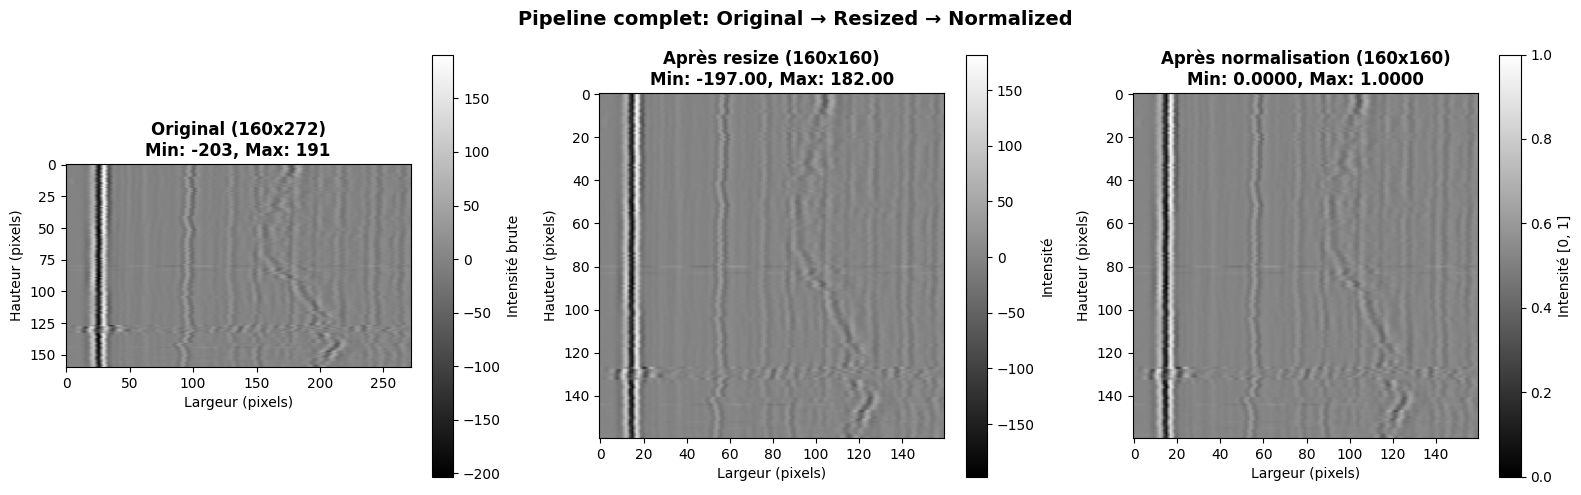
\includegraphics[width=0.6\textwidth]{Configuration/exemple_pipeline_complet_preprocessing.png}
    \caption{Pipeline complet de prétraitement : Original $\rightarrow$ Redimensionné $\rightarrow$ Normalisé}
    \label{fig:preprocessing_pipeline}
\end{figure}

